\documentclass[11pt]{article}
\usepackage{textcomp,bbding,subfig}
\usepackage{float,amssymb,amsmath,amsfonts,bm}
\usepackage{graphicx,cite}
\usepackage[]{natbib}
\def\style{apa}
\usepackage[usenames,pdftex,dvips]{color,xcolor}
\usepackage{multirow,tabulary,colortbl,array}
\usepackage[normalem]{ulem}
\usepackage[colorlinks,bookmarksopen,bookmarksnumbered,citecolor=blue,urlcolor=blue]{hyperref}
\usepackage{moreverb,setspace}
\usepackage{algpseudocode}
\usepackage{algorithm}
%
% Text layout
\topmargin -1.5cm
\oddsidemargin 0.0cm
\evensidemargin 0.0cm
\textwidth 16.5cm
\textheight 23.5cm
\setlength{\parindent}{0cm}

% Remove brackets from numbering in List of References
% \makeatletter \renewcommand\@biblabel[1]{} \makeatother
\makeatletter
\renewcommand{\@biblabel}[1]{\quad#1.}
\makeatother
% 
\allowdisplaybreaks[2]          % to accomodate long proofs spanning over pages
% 
% aliasis
\newcommand{\bs}{\boldsymbol}
\newcommand{\mean}[2]{\left\langle{#1}\right\rangle_{#2}}
\newcommand\numberthis{\addtocounter{equation}{1}\tag{\theequation}}
% 
% vectors and matrices
\newcommand{\vb}{\boldsymbol{b}}
\newcommand{\vc}{\boldsymbol{c}}
\newcommand{\vh}{\boldsymbol{h}}
\newcommand{\vv}{\boldsymbol{v}}
\newcommand{\vx}{\boldsymbol{x}}
\newcommand{\vw}{\boldsymbol{w}}
\newcommand{\vs}{\boldsymbol{s}}
% 
\newcommand{\md}{\boldsymbol{D}}
\newcommand{\mv}{\boldsymbol{V}}
\newcommand{\mh}{\boldsymbol{H}}
\newcommand{\mw}{\boldsymbol{W}}
\newcommand{\mx}{\boldsymbol{X}}
% 
% with hats or tildes
\newcommand{\vbt}{\tilde{\vb}}
\newcommand{\vct}{\tilde{\vc}}
\newcommand{\vht}{\tilde{\vh}}
\newcommand{\vvt}{\tilde{\vv}}
\newcommand{\vvp}{\vv^{\prime}}
\newcommand{\mwt}{\tilde{\mw}}
\newcommand{\vxt}{\tilde{\vx}}
\newcommand{\vhh}{\hat{\vh}}
\newcommand{\vvh}{\hat{\vv}}
% 
% xiaoran's edit
\newcommand{\xadd}[1]{\textcolor{blue}{#1}}
\newcommand{\xdel}[1]{\textcolor{red}{\sout{#1}}}
\newcommand{\xrpl}[2]{\xdel{#1}\xadd{#2}}
\newcommand{\xacc}[1]{\textcolor{ForestGreen}{#1}}
% 
% encoders
% vector or matrix
\newcommand{\vecEC}[1]{\boldsymbol{#1}}
% 
% decoders
\newcommand{\vecDC}[1]{\boldsymbol{\tilde{#1}}} 
% 
\newcommand{\xVO}{\boldsymbol{x}}         % the x vector, original
\newcommand{\xVR}{\boldsymbol{\tilde{x}}} % the x vector, recovered
\newcommand{\xSO}{x}                      % the x scaler, original
\newcommand{\xSR}{\tilde{x}}              % the x scaler, recovered
% 
% the vector of ones
\newcommand{\one}{\boldsymbol{1}}
% the diagnal matrix
\newcommand{\I}[1]{\boldsymbol{I}^{#1}}
% 
% parameters in the neural network
\newcommand{\Par}{\boldsymbol{\Theta}}
\newcommand{\pEC}{\boldsymbol{\theta}}
\newcommand{\pDC}{\boldsymbol{\tilde{\theta}}}
% 
% Loss function in Cross Entropy form
\newcommand{\LCE}[2]{#1\log{#2} + (1-#1)\log{(1-#2)}}
% 
% derivative
\newcommand{\DRV}[2]{\frac{d #1}{d #2}}
\newcommand{\DRC}[3]{\DRV{#1}{#2}\DRV{#2}{#3}}
\newcommand{\PDV}[2]{\frac{\partial #1}{\partial #2}}
\newcommand{\PDC}[3]{\PDV{#1}{#2}\PDV{#2}{#3}}
% 
% invers logit, aka. sigmoid function
\newcommand{\SGM}[1]{\frac{1}{1+e^{-#1}}}
% 
% assign to diagnoral
\newcommand{\diag}[1]{\text{diag} (#1)}
% 
% declarations
% argument of the minimum / maximum
\DeclareMathOperator*{\argmin}{arg\,min}
\DeclareMathOperator*{\argmax}{arg\,max}

% \pagestyle{headings}

% \author{Xiaoran Tong, Qin Lu} 
\doublespacing
\begin{document}
\title{A note on Boltzmann Machine, Restricted Boltzmann Machine, and Deep Belief Network}
\maketitle
\begin{flushleft}
  Xiaoran Tong\textsuperscript{1},
  Qin Lu\textsuperscript{1*},
  \\
  \bigskip
  \textbf{1} Department of Epidemiology and Biostatistics, Michigan State University, East Lansing, USA

  \vskip 50ex
  Correspondence: Qing Lu\\
  Department of Epidemiology and Biostatistics\\
  College of Human Medicine\\
  Michigan State University\\
  909 Fee Road\\
  East Lansing, MI 48824-1030\\
  qlu@msu.edu\\
\end{flushleft}

\clearpage
\begin{abstract}
  This research note covers the basics of Restricted Boltman Machine, a energy based, generative neural network.
\end{abstract}
\clearpage

\section{Boltzmann Machine}
\subsection{Concept}
A Boltzmann Machine (BM) is an engergy based model for binary data generation process, who views the observed data as the fraction of a physics system on display. In the complete system, the observed $P$ dimensional data is in fact the realization of its $P$ visible units, denoted by vector $\vv$, besides which there are presumably $Q$ hidden units holding unobserved data, denoted by vector $\vh$. All units are allowed to connect with each other to form mutual dependencies, as Figure \ref{fig:gbm} illustrates:
\begin{figure}[h]
  \centering
  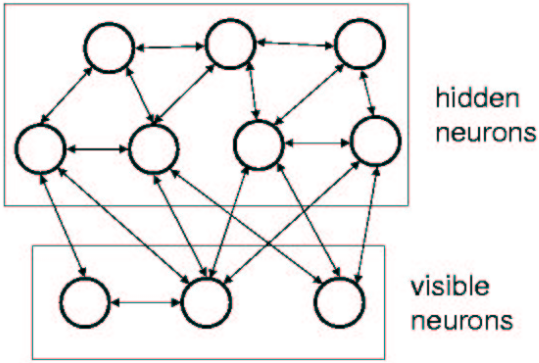
\includegraphics[width=200px]{img/gbm.png}
  \caption{Boltzmann Machine.}\label{fig:gbm}
\end{figure} \\
Together, the assignment of $\vv$ and $\vh$ comprices a complete $P+Q$ dimensional state vector $\vs =(\vv, \vh)$ of the system. Each distinct state is characterized by its energy, measurable by an energy function $E(\vs) = E(\vv, \vh)$. By the rule of nature, when a system reaches thermal equilibrium, states of lower engery are more likelly to sustain (thus more prevalent) than those of higher energy. Upholding this rule, the probability of a specific state $\vs=(\vv, \vh)$ presenting itself in the system, is proportional to the exponential of the negative energy of the said state, that is,
\begin{equation} \label{eq:p(s)}  % probability of observing a complete state
  \begin{split}
    \Pr(\vs) = \Pr(\vv, \vh) = \frac{e^{-E(\vv, \vh)}}{Z}, \quad Z = \int_{\vv,\vh} e^{-E(\vv, \vh) \,d\vv\,d\vh},
  \end{split}
\end{equation}
which is a Boltzmann distribution that assigns lower engery states higher density and vise versa. The partition function $Z$ serves as a normalizing constant to ensure $\int_{\vv, \vh} \Pr(\vv, \vh) \,d\vv\,d\vh = 1$. It is readily seen that engergy function $E(\vv, \vh)$ determines the system's dynamic behovior, it is therefore carefully choosen to allow emulation of the natural process that have given rise to the binary visible data we have collected. A Boltzmann Machine defines a binary system with energy function
\begin{align*}\label{eq:e(s)} % system energy for generic boltzmann machine
    E(\vv, \vh) = E(\vs) = -\sum_{i=1}^{P+Q} b_i s_i - \sum_{1 = i < j}^{P+Q} s_i w_{ij} s_j \numberthis
\end{align*}
where $b_i$ is an offest, serving as the energy thresholds to ``turn off'' the $i$ th unit $s_i$; $w_{ij}$ is the connection between the $i$ th and $j$ th units. The first term depicts that $s_i$ is more likely to stay ``on'' if $b_i$ is larger, because a system state that already has $s_i$ ``on'' demands lower energy to maintain (Eq.\,\ref{eq:e(s)}), it is therefore less likely for the system to jump out of such a state (Eq.\,\ref{eq:p(s)}); another way to see it, is that for the system to own a fair (50\%) chance of turning off $s_i$ under no interference form the other units, it must raise an extra $b_i$ energy. The second terms mode the mutual between $s_i$ and the others. Stronger connection promote binary agreement (when positive) or opposition (when negative) between $s_i$ and $s_j$, whereas weaker connection diminishes the mutual influcene between the two. The energy function is thus paramterized by $P+Q$ offsets and $P+Q \choose 2$ undirected connections, we represent them by $\pEC = \{b_i, m_{ij} | 1 \le i < j \le P+Q\}$. \\
A1: The probability of a particular unit $s_k, (k = 1, \dots, P+Q)$ being turned on in the next stage is, given the current state of the rest of the system $\vs_{k-}$:
\begin{equation}\label{eq:p(s_k=1)}
  \Pr(s_k = 1|\vs_{k-}) = \sigma(b_k + \sum_{i=1, i \ne k}^{P+Q}{s_i w_{ik}})
\end{equation}
Here,  $\sigma(x) = [1 + \exp({-x})]^{-1}$ is the sigmoid (logistic) function; $\vs_{k-}$ denote all units' value in the system, visible and hidden alike, except $s_k$. \\
Proof: start by splitting the energy contributed by the $k$ th unit from the rest,
\newcommand{\st}{\tilde{s}}
\begin{align*}
  E(\vs)
  & = \left( -\sum_{i=1, i \ne k}^{P+Q} b_i s_i - \sum_{1 \le i < j, i \ne k, j \ne k}^{P+Q} s_i w_{ij} s_j \right) + \left(-b_k s_k - \sum_{i=1, i \ne k}^{P+Q}s_i w_{ik} s_k \right) \\
  & = E(\vs_{-k}) + E(s_k), \\
  \Rightarrow \Pr(s_k | \vs_{k-})
  & = \int_{\vs_{-k}} \Pr(\vs) d\vs_{-k} = \frac{1}{Z} \int_{\vs_{-k}} e^{-E(\vs)} d\vs_{-k} \Leftarrow (\ref{eq:p(s)}) \\
  & = \frac{\int_{\vs_{-k}} e^{-E(\vs)} d\vs_{-k}}{\int_{\vs} e^{-E(\vs)} d\vs} \\
  & = \frac{e^{-E(s_k)} \int_{\vs_{-k}} e^{-E(\vs_{-k})} d\vs_{-k}}  {\int_{\st_k} \int_{\vs_{-k}} e^{-E(\vs_{-k})} d\vs_{-k}\,d\st_k} \\
  & = \frac{e^{-E(s_k)} \int_{\vs_{-k}} e^{-E(\vs_{-k})} d\vs_{-k}}  {[e^{-E(\st_k)}|_{\st_k=1} + e^{-E(\st_k)}|_{\st_k=0}] \int_{\vs_{-k}} e^{-E(\vs_{-k})} d\vs_{-k}} \\
  & = \frac{e^{-E(s_k)}}{e^{-E(\st_k)}|_{\st_k=1} + e^{-E(\st_k)}|_{\st_k=0}} \\
  % 
  \Rightarrow \Pr(s_k=1 | \vs_{k-})
  & = \frac{e^{-E(s_k)}|_{s_k=1}}{e^{-E(\st_k)}|_{\st_k=1} + e^{-E(\st_k)}|_{\st_k=0}} \\
  & = \frac{e^{b_k + \sum_{i=1, i \ne k}^{P+Q}{s_i w_{ik}}}}{e^{b_k + \sum_{i=1, i \ne k}^{P+Q}{s_i w_{ik}}} + e^{0}} \\
  & = \frac{1}{1 + e^{-b_k - \sum_{i=1, i \ne k}^{P+Q}{s_i w_{ik}}}} \\
  & = \sigma(b_k + \sum_{i=1, i \ne k}^{P+Q}{s_i w_{ik}})
\end{align*}
\subsection{MLE of Boltzmann Machine}
The best interest is to fine tune the flexible parameters $\pEC=\{b_i, w_{ij} | 1 \le i < j \le P+Q \}$ in such a way that the odds of observing the $N$ empirical data points $\mv=[\vv_1, \dots, \vv_N]^T$ on the visible units are maximized, which is equivalent to maximizing the marginal Boltzman distribution $\Pr(\vv, \vh)$ over assignments of $\vh$:
\begin{equation} \label{eq:p(v)}  % probability of observing a visible portion
  \begin{split}
    \Pr(\vv) = \int_{\vh}{\Pr(\vv, \vh)d\vh} = \frac{1}{Z} \int_{\vh}{e^{-E(\vv, \vh)}d\vh}.
  \end{split}
\end{equation}
The tuning requires the gradient of negative log likelihood with respect to $\pEC$ to decide updating rules, such that
\[ \pEC^{t+1} = \pEC^t + \epsilon \PDV{-\log{\Pr(\vv)}}{\pEC}, \]
where $\pEC^{t+1}$ is the resulting parameters of $t$ iterative updates, and $\epsilon$ is the learning rate. Now introduce the gradient expression:
\begin{align}\label{eq:gv1}
  -\PDV{\log{\Pr(\vv)}}{\pEC} &= -\PDV{\log{\int_{\vh}{e^{-E(\vv, \vh)}d\vh}}}{\pEC} + \PDV{\mean{\log{\int_{\vh}{e^{-E(\vvt, \vh)}d\vh}}}{\vvt}}{\pEC}.
\end{align}
The angled bracket $\mean{\dots}{\mx}$ denotes the expected value of an expression over random variable $\mx$.
There are a number of ways to interpret the gradient terms. The first term (without sign) is referred as \textbf{positive phase}, due to the fact that increases this term increases the likelihood of $\vv$; for the same reason, the second term (without sign) is called \textbf{negative phase}.\\
Derivation of (\ref{eq:gv1}):
\begin{align*}
  -\PDV{\log{\Pr(\vv)}}{\pEC}
  & = -\PDV{\log{\int_{\vh}{e^{-E(\vv, \vh)}d\vh}}}{\pEC} + \PDV{\log{\int_{\vvt, \vh} e^{-E(\vvt, \vh)} d\vvt\,d\vh }}{\pEC} \quad \Leftarrow (\ref{eq:p(s)}, \ref{eq:p(v)}) \\
  \textrm{\textbf{Positive phase:}} & \textrm{ Done!} \\
  \textrm{\textbf{Negative phase:}} \\
  \PDV{\log{\int_{\vvt, \vh} e^{-E(\vvt, \vh)} d\vvt\,d\vh }}{\pEC}
  & = \frac{1}{\int_{\vvt, \vh} e^{-E(\vvt, \vh)} d\vvt\,d\vh} \PDV{\int_{\vvt}\int_{\vh} e^{-E(\vvt, \vh)} d\vh\,d\vvt}{\pEC} \\
  & = \frac{1}{Z} \int_{\vvt} \PDV{ \int_{\vh}{e^{-E(\vvt, \vh)}}d\vh }{ \pEC } d\vvt \quad \Leftarrow (\ref{eq:p(s)}),\,\textrm{sum rule in deferenciation} \\
  & = \int_{\vvt}  \frac{1}{Z}\int_{\vh} e^{-E(\vvt, \vh)} d\vh \PDV{\log{\int_{\vh} e^{-E(\vvt, \vh) d\vh}}}{\pEC}  d\vvt \quad \Leftarrow \PDV{f(\vx)}{\vx}=f(\vx)\PDV{\log{f(\vx)}}{\vx} \\
  & = \int_{\vvt}{\Pr(\vvt) \PDV{\log{\int_{\vh}{e^{-E(\vvt, \vh)}d\vh}}}{\pEC}}d\vvt \quad \Leftarrow (\ref{eq:p(v)}) \\
  & = \mean{\PDV{\log{\int_{\vh}{e^{-E(\vvt, \vh)}d\vh}}}{\pEC}}{\vvt} \\
  & = \PDV{\mean{\log{\int_{\vh}{e^{-E(\vvt, \vh)}d\vh}}}{\vvt}}{\pEC} \quad (\textrm{Done!}).
\end{align*}
The above gradient form (\ref{eq:gv1}) is not ideal for direct implementation, since the update rule still involves gradient for both positive and negative phase, but it is meant for symbolic expression packages such as python theano which automatically program gradient function once the objective (or pseudo objective) function has been programmed. For low level implementation though, the update rules has to be gradient free, rearrange (\ref{eq:gv1}) we see
\begin{align*}
  \textrm{Positive Phase:}
  & \\
  \PDV{\log{\int_{\vh}{e^{-E(\vv, \vh)}d\vh}}}{\pEC} 
  & = \frac{1}{\int_{\vht} e^{-E(\vv, \vht)} d\vht}   \PDV{\int_{\vh} e^{-E(\vv, \vh)} d\vh}{\pEC}  \\
  & = \frac{1}{\int_{\vht} e^{-E(\vv, \vht)} d\vht}   \int_{\vh} \PDV{ e^{-E(\vv, \vh)}}{\pEC} d\vh \\
  & = \frac{1}{\int_{\vht} e^{-E(\vv, \vht)} d\vht}   \int_{\vh} e^{-E(\vv, \vh)}\PDV{-E(\vv, \vh)}{\pEC} d\vh \\
  & = \frac{1}{ \frac{1}{Z}  \int_{\vht} e^{-E(\vv, \vht)} d\vht}  \int_{\vh} \frac{e^{-E(\vv, \vh)}}{Z} \PDV{-E(\vv, \vh)}{\pEC} d\vh \\
  & = \frac{1}{\Pr(\vv)}  \int_{\vh} \Pr(\vv, \vh)\PDV{-E(\vv, \vh)}{\pEC} d\vh  & \Leftarrow (\ref{eq:p(s)})(\ref{eq:p(v)}) \\
  & = -\int_{\vh} \frac{\Pr(\vv, \vh)}{\Pr(\vv)} \PDV{E(\vv, \vh)}{\pEC} d\vh \\
  & = -\int_{\vh} \Pr(\vh | \vv) \PDV{E(\vv, \vh)}{\pEC}  d\vh \\
  & = -\mean{\PDV{E(\vv, \vh)}{\pEC}}{\vh|\vv} \\
  \textrm{Negative Phase:}
  & \\
  \PDV{\mean{\log{\int_{\vht}{e^{-E(\vvt, \vht)}d\vht}}}{\vvt}}{\pEC}
  &= \mean{\PDV{\log{\int_{\vht}{e^{-E(\vvt, \vht)}d\vht}}}{\pEC}}{\vvt} \\
  &= \mean{ -\mean{\PDV{E(\vvt, \vht)}{\pEC}}{\vht|\vvt}  }{\vvt} \\
  &= -\mean{\PDV{E(\vvt, \vht)}{\pEC}}{\vvt, \vht}.
\end{align*} 
Thus we could rewrite ({\ref{eq:gv1}) in terms of expected value:
\begin{align} \label{eq:gv2}
  -\PDV{\log{\Pr(\vv)}}{\pEC} = \mean{\PDV{E(\vv, \vh)}{\pEC}}{\vh|\vv} - \mean{\PDV{E(\vvt, \vht)}{\pEC}}{\vvt, \vht}
\end{align}
The gradients still exists on the right side, but it only involves energy function itself without either logarithm or exponentiation. The positive and negative phases (see \ref{eq:gv1}) are now re-expressed by two expectation terms, which is commonly referred as \textbf{data} phase and \textbf{model} phase, because the former is influenced by imperically observed data $\vv$ through conditioning, and the later entirely relying on a Boltzmann Machine runing freely without the interference of any substantial reality. From the above equation (\ref{eq:gv2}) we can now reinterprete the update rules by viewing the ``loss'' as the difference of expected energy between a system ``forced'' to generate observed $\vv$ on its $P$ visible units, and another system of identical topology but freely operate without any constraint. Therefore, minimizing this difference via its negative gradient w.r.t. machine parameters $pEC={\mw, \vb}$, amounts to urge the machine to generate $\vvt$ on its own, thus mimicking the nature process that had given rise to the training material we observed, and hopefully achieving satisfying generalization performance with the aid of hidden units.
Now, taking advantage of the simple form of energy function for a Boltzmann distribution (see \ref{eq:e(s)}), we immediately see
\begin{align} \label{eq:ge}
  \PDV{E(\vs)}{w_{ij}} = s_i s_j,  \quad \PDV{E(\vs)}{b_i} = s_i, \quad  (1 \le i < j \le P+Q)
\end{align}
Joint (\ref{eq:ge}) and (\ref{eq:gv2}) we get the primative update rules for the MLE of $\Pr(\vv)$:
\begin{align*} \label{eq:gv3}
  -\PDV{\log{\Pr(\vv)}}{w_{ij}} &= \mean{s_i s_j}{\vh|\vv} - \mean{s_i s_j}{\vvt, \vht} \\
  -\PDV{\log{\Pr(\vv)}}{b_i}    &= \mean{s_i}{\vh|\vv} - \mean{s_i}{\vvt, \vht} \numberthis \\
  \textrm{where }               & 1 \le i < j \le P+Q.
\end{align*}
The interpretation of update rules are quiet straight forward, for $w_{ij}$, the connection between $s_i$ and $s_j$, it is the difference of unit $i$ and $j$'s covariance between a system clumped on visible units and the same system that has been set free; as for $b_i$, the unit offset (activation threshold) of $s_i$, the update is the difference of mean value on the $i$ th unit, between a clumped and free run systems. At this point, we are readly to write the update algorithm of a Bolztmann Machine based on one sample:
\begin{algorithm}[h]
  \caption{One sample update rule for Boltzmann Machine}\label{alg:gbm1}
  \begin{algorithmic}[1]
    \State Clump $P$ dimenional obsevation on $P$ visible units $\vv$ \Comment{\textbf{Positive} Phase}
    \Repeat                                                           \Comment{burn in}
    \State one by one advance the state of $s_k$ if $s_k \in \vh$     \Comment{(Eq.\,\ref{eq:p(s_k=1)})}
    \Until{$\vh$ reaches thermal equilibrium}
    \Repeat                                                           \Comment{sampling}
    \State one by one advance the state of $s_k$ if $s_k \in \vh$     \Comment{(Eq.\,\ref{eq:p(s_k=1)})}
    \State Store $\vs=(\vv, \vh)$
    \Until{enough sample of $\vs$ is gathered}
    \State $\mean{s_i s_j}{\vh|\vv} \approx$ proportion of times both $s_i$ and $s_j$ are on
    \State $\mean{s_i}{\vh|\vv} \approx$ proportion of times $s_i$ is on
    \Statex

    \State Relex the constraint on $P$ visible units $\vv$            \Comment{\textbf{Negative} Phase}
    \Repeat                                                           \Comment{burn in}
    \State one by one advance the state of $s_k$                      \Comment{(Eq.\,\ref{eq:p(s_k=1)})}
    \Until{$\vs$ reaches thermal equilibrium}
    \Repeat                                                           \Comment{sampling}
    \State one by one advance the state of $s_k$                      \Comment{(Eq.\,\ref{eq:p(s_k=1)})}
    \State Store $\vs=(\vv, \vh)$
    \Until{enough sample of $\vs$ is gathered}
    \State $\mean{s_i s_j}{\vvt, \vht} \approx$ proportion of times both $s_i$ and $s_j$ are on
    \State $\mean{s_i}{\vvt, \vht} \approx$ proportion of times $s_i$ is on
    \Statex

    \State $-\Delta w_{ij} \gets \mean{s_i s_j}{\vh|\vv} - \mean{s_i s_j}{\vvt, \vht}$ 
    \State $-\Delta b_{i} \gets \mean{s_i}{\vh|\vv} - \mean{s_i}{\vvt, \vht}$ 
    \State \Return $-\Delta \mw$ and $-\Delta \vb$
  \end{algorithmic}
\end{algorithm} \\
Although the update rules has sample form, the exact values of $\mean{s_i s_j}{\vh|\vv}$, $\mean{s_i}{\vh|\vv}$, as well as $\mean{s_i s_j}{\vvt, \vht}$, $\mean{s_i}{\vvt, \vht}$, are computationally intractable because they involves going through either all $P+Q \choose 2$ states (for negative phase) or $Q \choose 2$ hidden states (for positive phase). Therefore we resolved to Gibbis sampling for approximations of the four mean values. Still, the sampling requires considerable time, and the resulting update rules is a noisy gradient of $\Pr(\vv)$ w.r.t. $\mw$ and $\vb$. Thus, Boltzmann Machine is unfit for problems involving large number of variables, a issue somewhat mitigated by relpacing the Gibbs sampling procedure with mean field approximation (will be included in this note in the future).
The expansion of the one sample update rule to a batch of $N$ samples is straight forward, just apply Algorithm \ref{alg:gbm1} to each sample then take the mean over $N$ sets of update rules.
% new subsection
\section{Restricted Boltzmann Machine}
\subsection{Concept}
In a Bolzmann Machine (BM), units are fully connected with each other, the preceding ``Restricted'' highlights additional constraints that connection is forbidden among visible units, as well as among hidden units, while full connection is still established between the two, see Figure \ref{fig:rbm} for an illustration.
\begin{figure}[h]
  \centering
  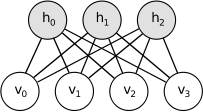
\includegraphics[width=100px]{img/rbm.png}
  \caption{The Restricted Boltzmann Machine.}\label{fig:rbm}
\end{figure} \\
Like the more general Boltzmann Machine (BM), the behavior of a RBM system is still determined by the engergy function $E(\vv, \vh)$ parameterized by $\pEC$, now thanks to the restriction however, the terms concerning visible and hidden units can be factored out from each other:
\begin{equation} \label{eq:rbm:e(s)}
  E(\vv, \vh) = -\sum_{i=1}^{P}{b_i v_i} - \sum_{j=1}^{Q}{c_j h_j} - \sum_{i=1}^P\sum_{j=1}^Q{v_i w_{ij} h_j} = -\vb^T \vv - \vc^T \vh - \vh^T \mw \vv,
\end{equation}
where $b_i$ tells the energy taken away from the system when the $i$ th visible units $v_i$ is ``on'' (or extra energy required in order to have a fair chance turning it off), that is, larger $b_i, (i=1, \dots, P)$ means lower total energy when $v_i$ is ``on'', making any state with $v_i=1$ more stable (i.e.,\,more likely to be observed); $c_j$ is interpreted quite the same, larger $c_j, (j=1, \dots, Q)$ make states having $h_j$ turned ``on'' relatively harder to turn away from, implying higher chance to observe $h_j=1$. As for the connection $w_{ij}$ between the $i$ th visible and $j$ th hidden units, visualized by the edges in Figure \ref{fig:rbm}, a large value either encourages (when positive) or prohibits (when negative) co-activation of $v_i$ and $h_j$, conversely, a small $w_{ij}$ diminish mutual dependency of the two.
\subsection{MLE for RBM}
Much like the BM, the goal of tuning a RBM is to maximum the chance of presenting $P$ dimensional emprical observations on its visible units, which is transfered into minimizing the marginal probability of an visible assignment $\vv$ in the the negative log scale. RBM shares the same gradient form with BM, both involve the intractable calculation of the expected values of a full Bolztmann distribution and its conditional form on observed values (equation \ref{eq:gv3}). However, exploitating the visible - visible and hidden - hidden independence (figure \ref{fig:rbm}), the thermal dynamics of a RBM can be simulated by batches instead of one dimension at a time (equation \ref{eq:p(s_k=1)}), which can drastically speed up the sampling procedure needed to approximate the aforementioned 4 expected values (Eq.\,\ref{eq:gv3}). The batch simulation of the complete system $\Pr(\vs)=\Pr(\vv, \vh)$ involves drawing all visible units given the hidden units, and all hidden units given the visible ones, in a manner of back and forth:
\begin{align*}
  \Pr(v_i=1|\vh) & = \sigma(b_i + \sum_{j=1}^Q{w_{ij} h_j}), \quad i = 1, \dots, P; \numberthis \label{eq:rbm:p(v|h)} \\
  \Pr(h_j=1|\vv) & = \sigma(c_j + \sum_{i=1}^P{v_i w_{ij}}), \quad j = 1, \dots, Q. \numberthis \label{eq:rbm:p(h|v)}
\end{align*}
The speed gain over a BM of the same number of units is readily seen from equation (Eq.\,\ref{eq:rbm:p(h|v)}), such that the sampling of hidden units during the positive phase can start right after clumping the $P$ visible units with empirical observation $\vv$, besides instantly reaching thermal equilibrium without any burn in, the positive phase only have to use the same equation to conduct sampling. Also for the negative phase, by allowing all visible units $v_i (i=1, \dots, P)$ to be sampled simultaneously (Eq.\,\ref{eq:rbm:p(v|h)}) and all hidden units vise versa (Eq.\,\ref{eq:rbm:p(h|v)}), the time needed to reach thermal equilibrium, as well as the sampling thereafter, are substantially shortened. \\
\textbf{Proof of (\ref{eq:rbm:p(v|h)}) and (\ref{eq:rbm:p(h|v)})}: \\
\newcommand{\jt}{\tilde{j}}
\newcommand{\wt}{\tilde{w}}
\newcommand{\bt}{\tilde{b}}
\newcommand{\ct}{\tilde{c}}
Consider the RBM a special case of the BM comprised of the same number of visible and hidden units while fixing all the connections $w_{ij}$ to zero if $s_i$ and $s_j$ are both visible or both hidden. Without loss of generality, let the $i$ th visible unit $v_i$ also be the $i$ th unit $s_i$ of the complete system $\vs=(\vv, \vh)$, where $i=1, \dots, P$; let the $\jt$ th hidden units $h_{\jt}$ be the $P+\jt$ th unit $s_{P+\jt}$ of the complete system, where $\jt=1, \dots, Q$; lastly, let $\wt_{i\jt}$ = $w_{i,P+\jt}$, $\bt_i = b_i$, and $\ct_{\jt} = b_{P+\jt}$, where $\wt$, $\bt$ and $\ct$ denotes connections and biases of the RBM while $w$ and $b$ denote the connection and bias in the corresponding BM.
\begin{align*}
  \Pr(s_i=1|s_{i-}) & = \Pr(v_i=1|v_{i-}, \vh)                                  & \Leftarrow (\textrm{relabeling}) \\
                    & = \Pr(v_i=1|\vh)                                          & \Leftarrow v_i \perp \vv_{i-}    \\
  \Pr(s_i=1|s_{i-}) & = \sigma(b_i + \sum_{j=1, j \ne i}^{P+Q}{w_{ij}s_j} )     & \Leftarrow (\ref{eq:p(s_k=1)})   \\
                    & = \sigma(b_i + \sum_{j=1, j \ne i}^P{w_{ij}s_j}
                      + \sum_{\jt=1}^{Q}{w_{i,P+\jt}s_{P+\jt}}) \\
                    & = \sigma(\bt_i + \sum_{j=1, j \ne i}^P{w_{ij}v_j}
                      + \sum_{\jt=1}^{Q}{\wt_{i\jt}h_{\jt}})                    & \Leftarrow (\textrm{relabeling}) \\
                    & = \sigma(\bt_i + \sum_{j=1, j \ne i}^P{0 v_j}
                      + \sum_{\jt=1}^{Q}{\wt_{i\jt}h_{\jt}})                    & \Leftarrow v_i \perp \vv_{i-} \\
                    & = \sigma(\bt_i + \sum_{\jt=1}^Q{\wt_{i\jt}h_{\jt}}) \\
  \Rightarrow \Pr(v_i=1|\vh) & = \sigma(\bt_i + \sum_{\jt=1}^Q{\wt_{i\jt}h_{\jt}})
\end{align*}
We are done with (\ref{eq:rbm:p(v|h)}), similar argument and the same relabeling can be applied for (\ref{eq:rbm:p(h|v)}). Again, through relabeling units' indices and forcing $w_{ij} \equiv 0$ whenever $s_i$ and $s_j$ are both visible or hidden, the primative update rules for the RBM, that is, the negative gradient of marginal log likelihood of $\vv$ w.r.t. the RBM parameters $\pEC=\{\vb, \vc, \mw\}$, can be seen as a degeneration from the rules (Eq.\,\ref{eq:gv3}) for a BM with the same number of visible and hidden units:
\begin{align*}
  -\PDV{\log{\Pr(\vv)}}{w_{ij}} & = \mean{v_i h_j}{\vh|\vv} - \mean{v_i h_j}{\vvt, \vht}; \\
  -\PDV{\log{\Pr(\vv)}}{b_i} & = \mean{v_i}{\vh|\vv} - \mean{v_i}{\vvt, \vht} = \mean{v_i}{\vv} - \mean{v_i}{\vvt, \vht}; \\
  -\PDV{\log{\Pr(\vv)}}{c_j} & = \mean{h_j}{\vh|\vv} - \mean{h_j}{\vvt, \vht}; \\
  \textrm{where } i & = 1, \dots, P;\, j = 1, \dots, Q.
\end{align*}

Now we are ready to write down the RBM training algorithm based on one sample:
\begin{algorithm}[h]
  \caption{One sample update rule for Restricted Boltzmann Machine}\label{alg:rbm1}
  \begin{algorithmic}[1]
    \State Clump $P$ dimenional obsevation on $P$ visible units $\vv$ \Comment{\textbf{Positive} Phase}
    \Repeat                                                           \Comment{sampling without burn in}
        \State batch advance the state of all $h_j$                   \Comment{(Eq.\,\ref{eq:rbm:p(h|v)})}
        \State Store $\vh$
    \Until{enough sample of $\vh$ is gathered}
    \State $\mean{v_i h_j}{\vh|\vv} \approx$ proportion of times both $v_i$ and $h_j$ are on
    \State $\mean{v_i}{\vh|\vv}$ (or $\mean{v_i}{\vv}$) $\gets$ proportion of times $v_i$ is on\textsuperscript{1}
    \State $\mean{h_j}{\vh|\vv} \approx$ proportion of times $h_j$ is on
    \Statex

    \State Relex the constraint on $P$ visible units $\vv$            \Comment{\textbf{Negative} Phase}
    \Repeat                                                           \Comment{burn in}
        \State batch advance the state of all $h_j$                   \Comment{(Eq.\,\ref{eq:rbm:p(h|v)})}
        \State batch advance the state of all $v_i$                   \Comment{(Eq.\,\ref{eq:rbm:p(v|h)})}
    \Until{$\vs=(\vv, \vh)$ reaches thermal equilibrium}
    \Repeat                                                           \Comment{sampling}
        \State batch advance the state of all $h_j$                   \Comment{(Eq.\,\ref{eq:rbm:p(h|v)})}
        \State batch advance the state of all $v_i$                   \Comment{(Eq.\,\ref{eq:rbm:p(v|h)})}
    \Until{enough sample of $\vs$ is gathered}
    \State $\mean{v_i h_j}{\vvt, \vht} \approx$ proportion of times both $v_i$ and $h_j$ are on
    \State $\mean{v_i}{\vvt, \vht} \approx$ proportion of times $v_i$ is on
    \State $\mean{h_j}{\vvt, \vht} \approx$ proportion of times $h_j$ is on
    \Statex

    \State $-\Delta w_{ij} \gets \mean{v_i h_j}{\vh|\vv} - \mean{v_i v_j}{\vvt, \vht}$
    \State $-\Delta b_{i} \gets \mean{v_i}{\vh|\vv} - \mean{v_i}{\vvt, \vht}$
    \State $-\Delta c_{j} \gets \mean{h_j}{\vh|\vv} - \mean{h_j}{\vvt, \vht}$
    \State \Return $-\Delta \mw$, $-\Delta \vb$, and $-\Delta \vc$
  \end{algorithmic}
\end{algorithm} \\
% 
\section{MLE with Symbolic Library}
The primative update rules are necessary for developing a BM trainer from scratch, in case of available symbolic mathematics libraries however, such as Python-Theano and Matlab-Symbolic, it is often unnecessary, or even over-developing to implement the primative rules in equation (\ref{eq:gv3}) directly. Instead, it would be more efficient and easier to just construct a crude objective function, let the software packages to figure out the gradient function, and subsequently, the update rules.
Review the negative log likelihood gradient in equation (\ref{eq:gv1}), we see the crude objective function to be minimized with respect to $\pEC$ is
\begin{align}\label{eq:l(v)1}
  -\log{\Pr(\vv)} = -\log{\int_{\vh}{e^{-E(\vv, \vh)}d\vh}} + \mean{\log{\int_{\vh}{e^{-E(\vvt, \vh)}d\vh}}}{\vvt}
\end{align}
which involves the mean of marginal distribution $\Pr(\vvt)$, posing a severe challenge to direct evaluation attempt, we instead resort to approximation via limited sampling from $\Pr(\vvt)$:
\begin{align}\label{eq:l(v)2}
  -\log{\Pr(\vv)} \approx -\log{\int_{\vh} e^{-E(\vv, \vh)} d\vh} + \frac{1}{|M|}\sum_{\vvt \in M}{\log{\int_{\vh} e^{-E(\vvt, \vh)}d\vh}}
\end{align}
where $M$ is the set of samples drawn from $\Pr(\vvt)$. \\
\subsection{Free Energy}
It is now helpfult to introduce the notion of ``\textbf{free energy}'' $F$, which, just likes the complete energy $E$ that corresponds to each distinct state $\vs=(\vv, \vh)$, corresponds to every distinct visible state $\vv$. \textbf{Free energy} takes the form:
\begin{align}\label{eq:f(v)}
    F(\vv) = -\log{\int_{\vh}{e^{-E(\vv, \vh)}d\vh}}.
\end{align}
Compare (\ref{eq:f(v)}) with (\ref{eq:e(s)}), we see that $F(\vv)$ in essence is the kernel of $\Pr(\vv)$ under negative log scale, which is the marginal distribution of $Pr(\vv, \vh)$ over $\vh$. Refer to equation (\ref{eq:p(s)}), $F(\vv)$ governs the system behavior in a similar manner, allbeit the only concern of $F(\vv)$ is the visible units:
\begin{align}\label{eq:p(v)|fe}
    \Pr(\vv) = \frac{e^{-F(\vv)}}{Z}, \quad\quad Z=\int_{\vv}{e^{-F(\vv)}}d\vv
\end{align}
It makes the aforementioned crude objective function expression more concise:
\begin{align}\label{eq:l(v)3}
  -\log{\Pr(\vv)} \approx F(\vv) - \frac{1}{|M|}\sum_{\vvt \in M}{F(\vvt)},
\end{align}
The update rules depends on the gradient of objective function with respect to the flexible parameters $\pEC$:
\begin{align}\label{eq:gv4}
  -\PDV{\log{\Pr(\vv)}}{\pEC} \approx \PDV{F(\vv)}{\pEC} - \PDV{\frac{1}{|M|}\sum_{\vvt \in M}{F(\vvt)}}{\pEC},
\end{align}
The negative log kernel of marginal probability $Pr(\vv)$, that is, the free energy, is simplified in a RBM:
\begin{align*}
  F(\vv) &= -\log{\sum_{\vh\in \{0,1\}^Q}{e^{\vb^T \vv + \vc^T \vh + \vh^T \mw \vv}}} \\
         &= -\log{\left[ e^{\vb^T\vv}\sum_{\vh\in \{0,1\}^Q}{e^{\vh^T(\vc + \mw \vv)}} \right]} \\
         &= -\vb^T\vv - \log{\sum_{\vh\in \{0,1\}^Q}{ \prod_{j=1}^Q{e^{h_j(c_j + \vw_j\vv)}} }}; \\
  \textrm{and} \quad & \sum_{h_1, \dots h_Q \in \{0,1\}}{\prod_{j=1}^Q{e^{h_j(c_j + \vw_j\vv)}}} \\
         &= (e^{c_1+\vw_1\vv}+e^{0}) \sum_{h_2 \dots h_Q \in\{0,1\}}{ \prod_{j=2}^Q{e^{h_j(c_j + \vw_j\vv)}} } \\
         &= (e^{c_1+\vw_1\vv}+e^{0})(e^{c_2+\vw_2\vv}+e^{0}) \sum_{h_3 \dots h_Q \in\{0,1\}}{ \prod_{j=3}^Q{e^{h_j(c_j + \vw_j\vv)}} } \\
         & \quad \vdots \\
         &= (e^{c_1+\vw_1\vv}+e^{0})(e^{c_2+\vw_2\vv}+e^{0}) \dots (e^{c_Q+\vw_Q\vv}+e^{0}) \\
         &= \prod_{j=1}^Q{(e^{c_j+\vw_j\vv} + 1)}; \\
  \Rightarrow
  F(\vv) &= -\vb^T\vv - \sum_{j=1}^Q{\log{(e^{c_j+\vw_j\vv} + 1)}} \numberthis \label{eq:fe_bin}.
\end{align*}
A symbolic library user should program the \textbf{free energy} function $F(\vv)$, the sampling procedure from $\Pr{\vv}$, the approximated crude lose (equation \ref{eq:l(v)3}), but leave the code of gradient function (equation \ref{eq:gv4}) for the library to automatically program, optimize, and even compile into low level machine language for best hardware utilization.
%
\singlespacing 
\bibliographystyle{\style}
\bibliography{ref}

\end{document}

%%% Local Variables:
%%% mode: latex
%%% TeX-master: t
%%% End:
